\chapter{Proceso de optimización del código}  \label{apendice:optimizacion_codigo}

Como ya se ha comentado en la \sectionref{isec:planificacion}, una parte esperada del proceso de desarrollo es encontrar problemas de rendimiento, localizar qué partes del código están produciendo los problemas, y re-escribir implementaciones mucho más eficientes.

Además, en \sectionref{isubs:localizacion_partes_criticas} hemos justificado por qué es necesario realizar un \textit{profile} para identificar las secciones críticas del código. De otra forma, estaríamos realizando optimizaciones con muy poco impacto.

En este apéndice explicamos en detalle cómo hemos desarrollado todo este proceso, paso a paso.

\section{Identificación del problema}

Identificamos problemas con los tiempos de cómputo por primera vez trabajando con el \textit{dataset} \textit{LFW}. El proceso de identificación y resolución se agrupan en las issues \cite{informatica:issue35_profiling} y \cite{informatica:issue36_slowmetrics}. Todo el proceso de optimización se resuelve en la \textit{pull request} \cite{informatica:pr42_profiling}. El \textit{commit} \lstinline{6aade342e07} \cite{informatica:commit_base_optimizacion} indica el estado original previo a realizar el proceso de optimización (\textit{profiling}, identificación de cuellos de botella, \textit{benchmarking} y cambios en las implementaciones).

\section{Organización del proceso}

El proceso de optimización se compone de los siguientes pasos:

\begin{itemize}
	\item \textit{Profiling} del código. Usamos la librería \lstinline{cProfile}. Esta forma parte de la librería estándar de \lstinline{Python}.
	\item Identificación de los cuellos de botella. Para ello usaremos \lstinline{pstats} (que también forma parte de la librería estándar de \lstinline{python}) para explorar los resultados desde la terminal, y \lstinline{snakeviz} para explorar los datos de forma gráfica e interactiva.
	\item Introducción de \textit{benchmarks} para medir los tiempos de ejecución en los cuellos de botella que vamos a modificar. Con ello tendremos mayor control sobre el impacto que suponen los cambios introducidos.
	\item Realización de cambios sobre los cuellos de botella identificados y medición el impacto que suponen.
\end{itemize}

En la sección de código donde realizamos el entrenamiento, añadimos la opción de usar la librería \lstinline{cProfile} para generar un \textit{profile}. Guardamos los resultados en la carpeta \lstinline{./src/profiling}, en los archivos \lstinline|{first, second, third}_profile.stat|.

Usando el paquete \lstinline{pstats} podemos realizar consultas sobre los archivos \lstinline{.stat}. Para ello usamos el comando \lstinline{python -m pstats <file_path>}. Tomamos el tiempo acumulado de cada función y guardamos los resultados en los archivos \lstinline|{first, second, third}_profile.txt|. Usando un editor de texto, filtramos esos archivos para que solo contengan entradas asociadas a funciones de nuestra librería (no nos interesan los tiempos de funciones de la librería estándar, por ejemplo) y guardamos el filtrado en los archivos \lstinline|{first, second, third}_profile_filtered.txt|. Con ello, podemos consultar estos resultados filtrados con un editor de texto, de forma más cómoda que trabajando con todos los resultados usando \lstinline{pstats}.

Usando el paquete \lstinline{snakeviz} podemos consultar de forma gráfica e interactiva los resultados almacenados en los archivos \lstinline{.stat}. Esto permite explorar los resultados de forma mucho más intuitiva, como veremos a continuación.

\section{Primer \textit{profile}}

En este \textit{profile} usamos los siguientes parámetros durante el ciclo de entrenamiento:

\begin{itemize}
	\item Enfoque \textit{lazy} para el aumentado de datos (véase el \sectionref{isec:aumentado_datos}).
	\item $P = 200$, $K = 2$.
	\item Dimensión del \textit{embedding} a aprender igual a 5.
\end{itemize}

Visualizamos los resultados con \lstinline{snakeviz} en la \imgref{img:optimizacion_01}.

\begin{figure}[!hbtp]
	\centering
	\ajustarsubcaptions

	\begin{subfigure}{.5\textwidth}
		\centering
		\includegraphics[width=0.9\linewidth]{informatica/profiles/first_profile/global}
		\caption{Visualización global de todo el proceso de entrenamiento}
		\label{img:first_profile_global}
	\end{subfigure}%
	\begin{subfigure}{.5\textwidth}
		\centering
		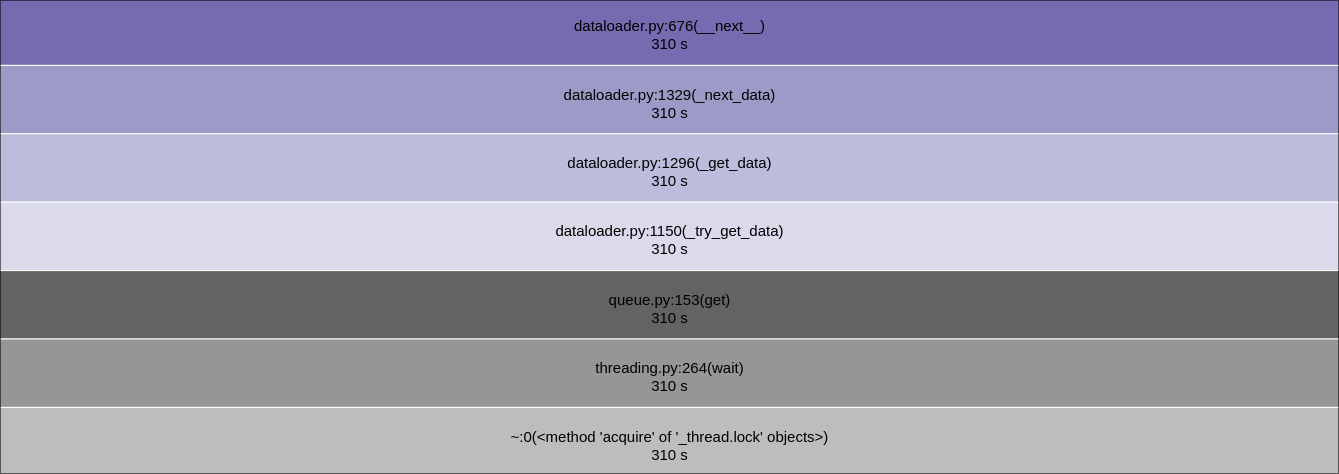
\includegraphics[width=0.9\linewidth]{informatica/profiles/first_profile/dataloader}
		\caption{Visualización de los tiempos involucrados en computar \lstinline{dataloader.__next__}}
		\label{img:first_profile_dataloader_next}
	\end{subfigure}
	\caption{Visualizaciones obtenidas usando \lstinline{snakeviz} para los resultados del \textit{profile} inicial}
	\label{img:optimizacion_01}
\end{figure}

El tiempo total de cómputo es de 328.638 segundos. Podemos ver en la \imgref{img:first_profile_global} que la mayor parte del tiempo de entrenamiento se dedica al método \lstinline{dataloader.__next__()}. En la \imgref{img:first_profile_dataloader_next} podemos ver que, en dicho método, prácticamente todo el tiempo estamos esperando a que se complete una operación asíncrona, como indica \lstinline{threading.wait()}.

Creemos que esto es por estar empleando el enfoque \textit{lazy} para el aumentado de datos. Cada vez que queremos acceder a una nueva imagen, tenemos que generarla en ese preciso instante. Por tanto, en la siguiente iteración no usaremos el enfoque \textit{lazy}. Veremos si los tiempos aumentan o disminuyen, y si aparecen nuevas partes de código a optimizar.

\section{Segundo \textit{profile}}

Como ya hemos comentado, esta vez nos centraremos en usar un enfoque no \textit{lazy} para el aumentado de datos. Si intentamos usar los mismos valores $P = 200$, $K = 2$, saturamos la memoria del proceso haciendo que este aborte. Así que tenemos que usar $P = 100, K = 2$, lo que supone un problema para comparar los nuevos resultados con los del primer \textit{profile}.

Para evitar que estas diferencias al cambiar los parámetros $\{P, K\}$ interfieran en nuestra optimización, lanzamos las dos versiones (\textit{lazy} y clásico) usando los valores $P = 100$, $K = 2$, y con ello podremos comparar de forma justa los tiempos de ejecución. Los resultados se resumen en la \tableref{table:optimizacion_01}.

\begin{table}[!hbtp]
	\centering
	\begin{tabular}{|l|l|l|}
		\hline
		\textbf{Enfoque} & \textbf{Tiempo total de ejecución (s)} & \textbf{Tiempo total de ejecución (min)} \\
		\hline

		\textit{Lazy}    & 952.00s                                & 15.86 min                                \\
		Clásico          & 917.84s                                & 15.29 min                                \\

		\hline
	\end{tabular}
	\caption{Tiempos de ejecución de los dos enfoques de aumento de datos, usando los valores $P = 100, K = 2$}
	\label{table:optimizacion_01}
\end{table}

Como era de esperar por lo comentado en el \sectionref{isec:aumentado_datos}, el enfoque \textit{lazy} conlleva un tiempo de ejecución mayor. Solo estamos midiendo el tiempo de ejecución en el entrenamiento, no tenemos en cuenta los tiempos asociados a generar el \textit{dataset} aumentado. Y de esta forma, el enfoque clásico ya tiene todas las imágenes pre-computadas (lo que conlleva un tiempo considerable que no estamos teniendo en cuenta), mientras que el enfoque \textit{lazy} las tiene que generar a demanda. Sin embargo, acabamos de ver que el enfoque \textit{lazy} permite usar valores $\{P, K\}$ más altos. Y además, la diferencia no es demasiado grande: menos de un minuto de diferencia en tiempos totales de algo más de 15 minutos (sin considerar lo que tarda en generarse el \textit{dataset} aumentado de forma clásica).

Una vez resuelto esto, realizamos un segundo \textit{profile} usando los siguientes parámetros:

\begin{itemize}
	\item $P = 100$, $K = 2$.
	\item Aumentado de datos clásico.
	\item Dimensión del \textit{embedding} aprendido igual a 5.
\end{itemize}

Los resultados del segundo \textit{profile} se muestran en la \imgref{img:optimizacion_02}. En este caso, podemos ver que los resultados ya son más interesantes. Los tiempos de entrenamiento se dividen principalmente en dos bloques: el asociado a mostrar métricas con nuestra estructura de \textit{logging} (véase el \sectionref{isec:loggin_metricas}) y el asociado al cálculo de la función de pérdida. Empecemos viendo el bloque de los \textit{loggers}, en la \imgref{img:second_profile_tiempos_metricas}.

\begin{figure}[!hbtp]
	\centering
	\includegraphics[width=0.8\textwidth]{informatica/profiles/second_profile/global}
	\caption{Visualización obtenida usando \lstinline{snakeviz} para los resultados del segundo \textit{profile}}
	\label{img:optimizacion_02}
\end{figure}

\begin{figure}[!hbtp]
	\centering
	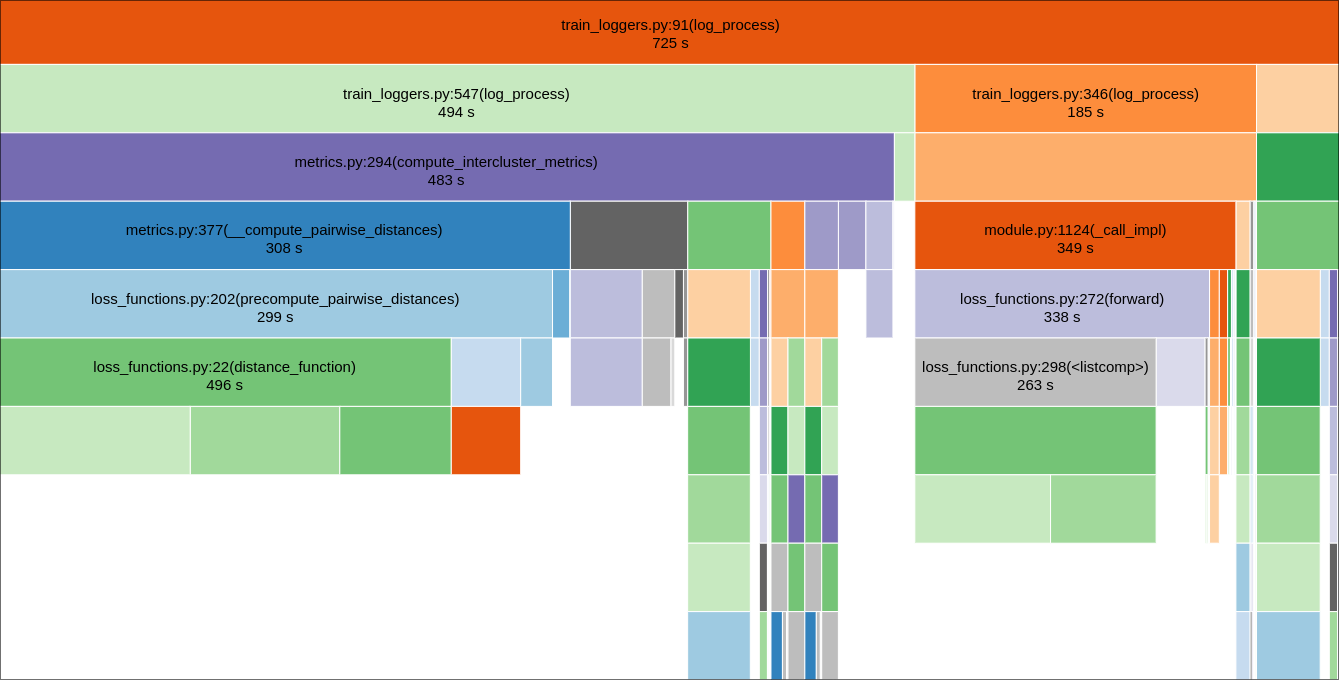
\includegraphics[width=0.8\textwidth]{informatica/profiles/second_profile/loggers}
	\caption{Visualización de los tiempos de cómputo asociados al \textit{logging} de métricas}
	\label{img:second_profile_tiempos_metricas}
\end{figure}

Podemos ver que la mayoría de tiempo se pasa en \lstinline{compute_intercluster_metrics} (métrica que introducimos en la \sectionref{isubs:teoria_distancia_intra_inter_cluster}). Un gran porcentaje del tiempo de esta última función se gasta en pre-computar las distancias entre todos los pares de individuos. A su vez, gran parte del tiempo se gasta en computar la función de distancia \lstinline{distance_function} entre todos los pares de \textit{embeddings}.

Ahora estudiamos el bloque asociado al cálculo de la función de pérdida, en la \imgref{img:optimizacion_03}. Podemos ver que la mayor parte del tiempo se pasa en realizar una comprensión de lista (análogo a un bucle \lstinline{for}) para computar distancias entre todos los pares de puntos, como ya hemos visto en la \imgref{img:second_profile_tiempos_metricas}.

\begin{figure}[!hbtp]
	\centering
	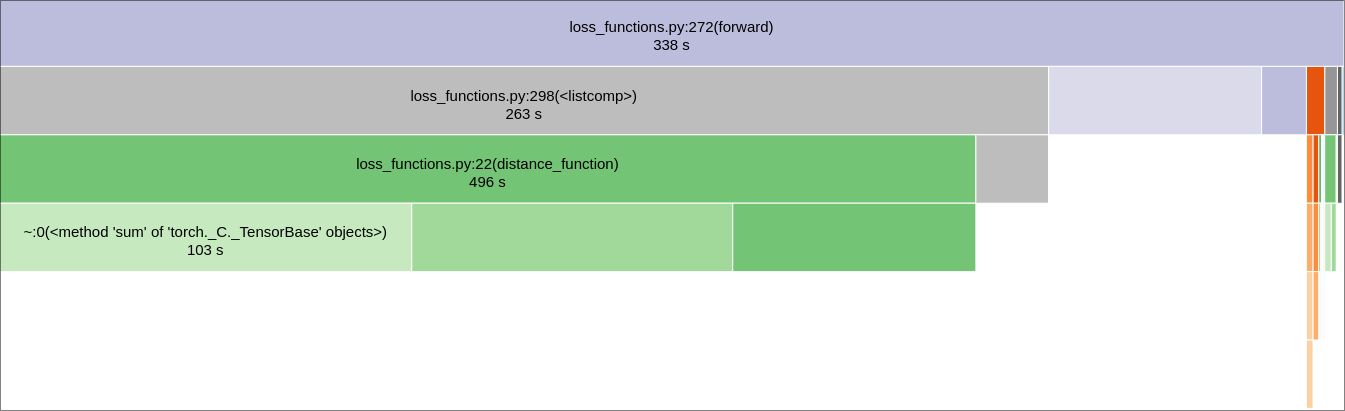
\includegraphics[width=0.8\textwidth]{informatica/profiles/second_profile/loss_function}
	\caption{Visualización de los tiempos de cómputo asociados al cálculo de la función de pérdida}
	\label{img:optimizacion_03}
\end{figure}

\section{Primera ronda de optimizaciones}

Con toda esta información, hemos localizado algunos cuellos de botella. Escribimos \textit{benchmarks} para estas partes del código previo a introducir cambios. Gracias a disponer de \textit{benchmarks}, estudiamos si estos cambios mejoran o empeoran los tiempos de cómputo.

Algunos detalles sobre los \textit{benchmarks}:

\begin{itemize}
	\item Estudiaremos los tiempos de ejecución de las funciones \lstinline{compute_intercluster_metrics} y \lstinline{precompute_pairwise_distances} con los dos \textit{scripts} que se encuentran en \lstinline{./src/benchmarks}.
	\item Correremos estos \textit{scripts} en la plataforma \textit{Google Colab} (véase la \sectionref{isec:entorno_ejecucion}), usando un \textit{Notebook} que invoca el código de los \textit{benchmarks}: \lstinline{./src/benchmarks/Benchmarking notebook.ipynb}.
	\item Usaremos los parámetros:
	      \begin{itemize}
		      \item $P = 100, K = 2$.
		      \item Enfoque \textit{lazy} para el aumentado de datos.
		      \item Dimensión del \textit{embedding} a aprender igual a 5.
		      \item Una época de entrenamiento.
	      \end{itemize}
\end{itemize}

La siguiente tabla muestra los cambios introducidos y los tiempos de los \textit{benchmarks}. Además, mostramos el tiempo de ejecución del \textit{Notebook} \lstinline{LFW Notebook.ipynb}, que en el momento de realizar las optimizaciones, usábamos para entrenar y validar modelos sobre el \textit{dataset} \textit{LFW}.

\begin{table}[!hbtp]
	\centering
	\scalebox{0.8}{
		\begin{tabular}{lccccc}
			\toprule
			\textbf{}           & \multicolumn{2}{c}{\textbf{\lstinline|compute_intercluster_metrics|}} & \multicolumn{2}{c}{\textbf{\lstinline|precompute_pairwise_distances|}} & \textbf{Tiempo entrenamiento}                         \\
			\cmidrule(lr){2-3} \cmidrule(lr){4-5}
			\textbf{Id. Cambio} & Media                                                                 & Desv. Típica                                                           & Media                         & Desv. Típica &        \\
			\midrule
			1                   & 16.01                                                                 & 2.41                                                                   & 37.02                         & 0.56         & 939.52 \\
			2                   & 3.25                                                                  & 0.93                                                                   & 12.05                         & 0.67         & 734.75 \\
			3                   & 2.55                                                                  & 1.61                                                                   & 12.75                         & 1.48         & 625.89 \\
			\bottomrule
		\end{tabular}
	}
	\caption{Tabla que recoge el proceso de optimización del código. Identificamos numéricamente los cambios realizados, que a continuación describiremos. Por cada cambio, vemos los nuevos resultados en los \textit{benchmarks}. También vemos el tiempo que tarda en completarse el ciclo de entrenamiento. Los tiempos de los \textit{benchmarks} se dan como un par (media, desviación típica). Damos los tiempos en segundos}
\end{table}

Los cambios realizados asociados a los identificadores numéricos son:

\begin{enumerate}
	\item Estado inicial de la base de código. No se han realizado cambios todavía. Los tiempos en este estado se toman como base a mejorar.
	\item En \lstinline|precompute_pairwise_distances|, usamos el método \lstinline|cdist| de \lstinline|pytorch| para calcular una matriz de distancias. Convertimos dicha matriz a un diccionario para respetar la interfaz que ciertas clases esperan de esta función.
	\item Usamos \lstinline|precompute_pairwise_distances| en el cálculo de las funciones de pérdida. Introducimos algunos pre-cómputos en \lstinline|compute_intracluster_distances| para acelerar la ejecución.
\end{enumerate}

Podemos ver que los cambios introducidos mejoran los tiempos de cómputo de forma sustancial. Por tanto, estos cambios son relevantes y los mantenemos, aunque esto implique que algunas funciones sean más complicadas y menos legibles.

\section{Tercer \textit{profile}}

La primera ronda de optimizaciones potencialmente ha cambiado los cuellos de botella del código. Así que es necesario llevar a cabo un tercer \textit{profile} para estudiar el estado de la base de código e identificar, si hiciera falta, nuevos cuellos de botella a optimizar.

En este \textit{profile} usamos los siguientes parámetros:

\begin{itemize}
	\item $P = 100$, $K = 2$.
	\item Una época de entrenamiento.
	\item \textit{Embedding Dimension} = 1.
	\item Enfoque \textit{Lazy} para el aumentado de datos.
\end{itemize}

Visualizamos los resultados del \textit{profile} en la \imgref{img:optimizacion_04}. Podemos ver que la mayor parte del tiempo se corresponde al \textit{logging} de métricas, seguido del acceso a los datos. Sobre el acceso de datos ya hemos trabajado, así que pasamos a estudiar en qué se gasta el tiempo en el \textit{logging}, en la \tableref{table:optimizacion_02}.

\begin{figure}[!hbtp]
	\centering
	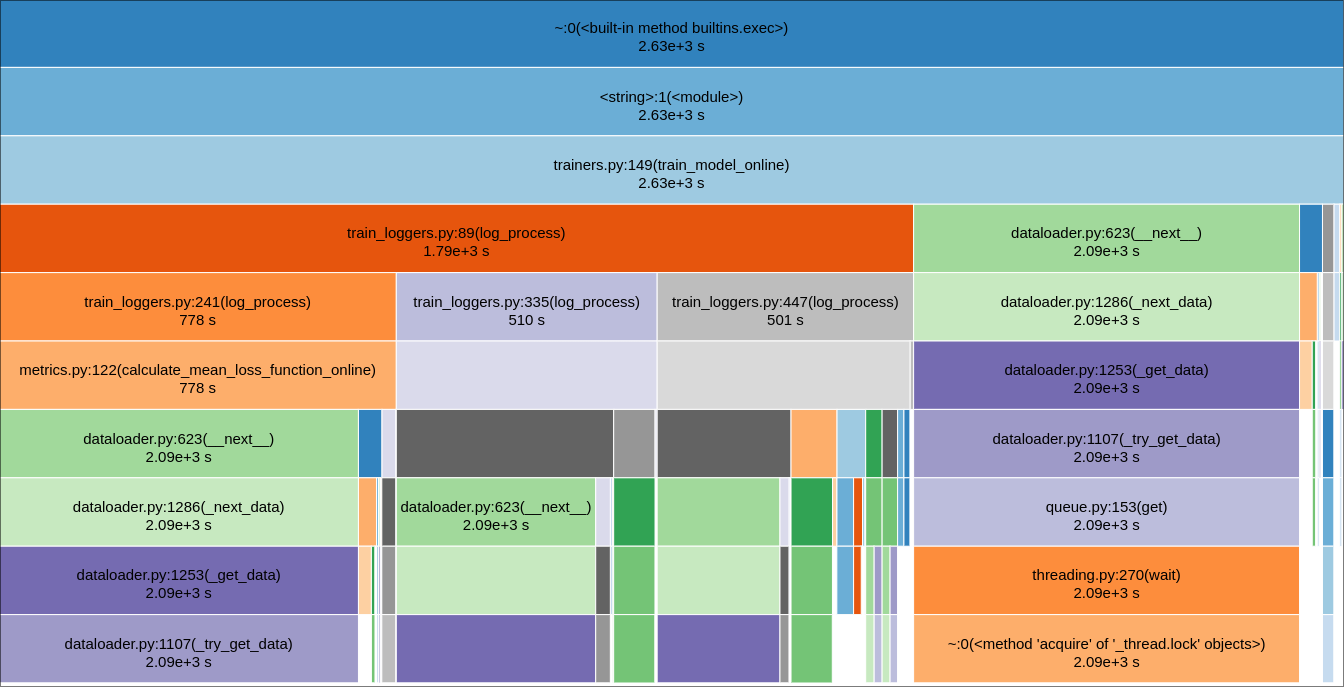
\includegraphics[width=0.8\textwidth]{informatica/profiles/third_profile/total}
	\caption{Visualización global de todo el proceso de entrenamiento.}
	\label{img:optimizacion_04}
\end{figure}

\begin{figure}[!hbtp]
	\centering
	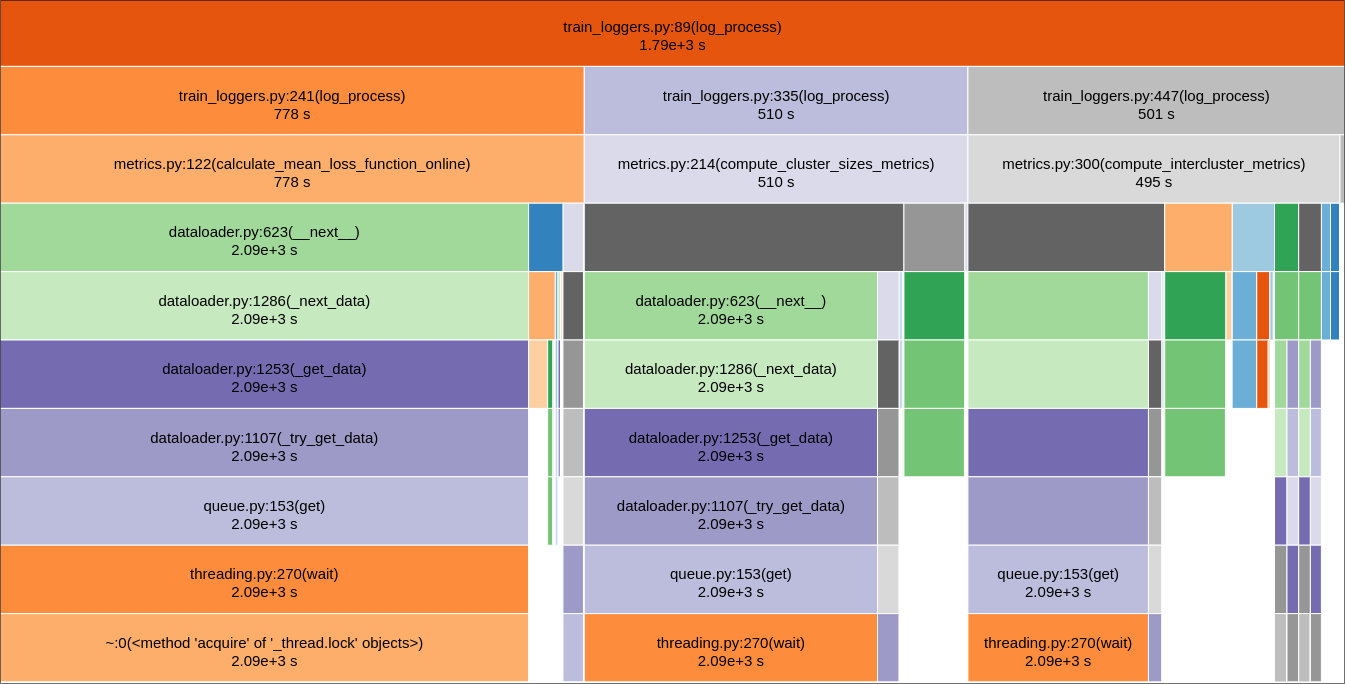
\includegraphics[width=0.8\textwidth]{informatica/profiles/third_profile/logging}
	\caption{Visualización de los tiempos de cómputo asociados al \textit{logging} de métricas}
	\label{table:optimizacion_02}
\end{figure}

Tenemos tres bloques, que podemos expandir, como mostramos en la \imgref{img:optimizacion_05}. En base a estas visualizaciones podemos ver que:

\begin{sloppypar}
	\begin{itemize}
		\item Las tres métricas que en ese momento estábamos mostrando suponen aproximadamente la misma cantidad de tiempo.
		\item En \lstinline{calculate_mean_loss_function_online}, la mayor parte del tiempo se debe al acceso a los datos.
		\item En \lstinline{compute_cluster_sizes_metrics}, la mayor parte del tiempo se pasa en \lstinline{__get_portion_of_dataset_and_embed}.
		\item En \lstinline[breaklines=true]{compute_inter_cluster_metrics} la mayor parte del tiempo se pasa en \lstinline[breaklines=true]{__get_portion_of_dataset_and_embed}, pero no tanto como en el caso anterior. Le sigue la función \lstinline{__compute_pairwise_distances}.
	\end{itemize}
\end{sloppypar}

\begin{figure}[!hbtp]
	\centering
	\begin{subfigure}{.5\textwidth}
		\centering
		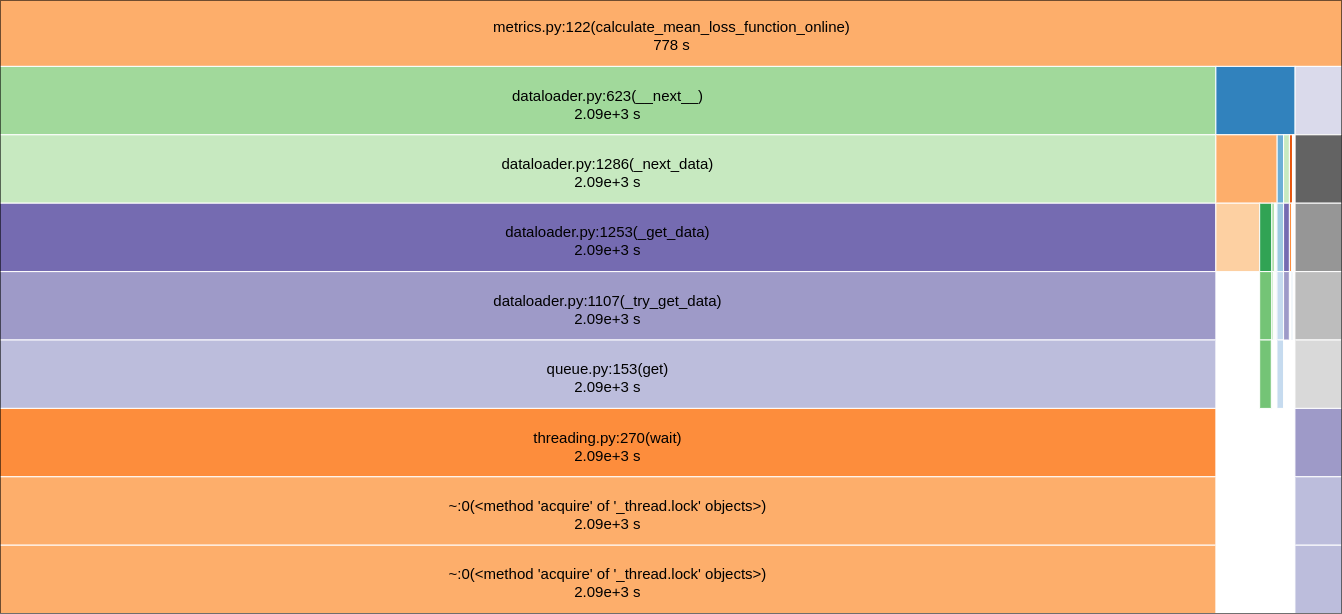
\includegraphics[width=0.98\linewidth]{informatica/profiles/third_profile/logging_primero}
		\caption{\lstinline{calculate_mean_loss_function_online}}
	\end{subfigure}%
	\begin{subfigure}{.5\textwidth}
		\centering
		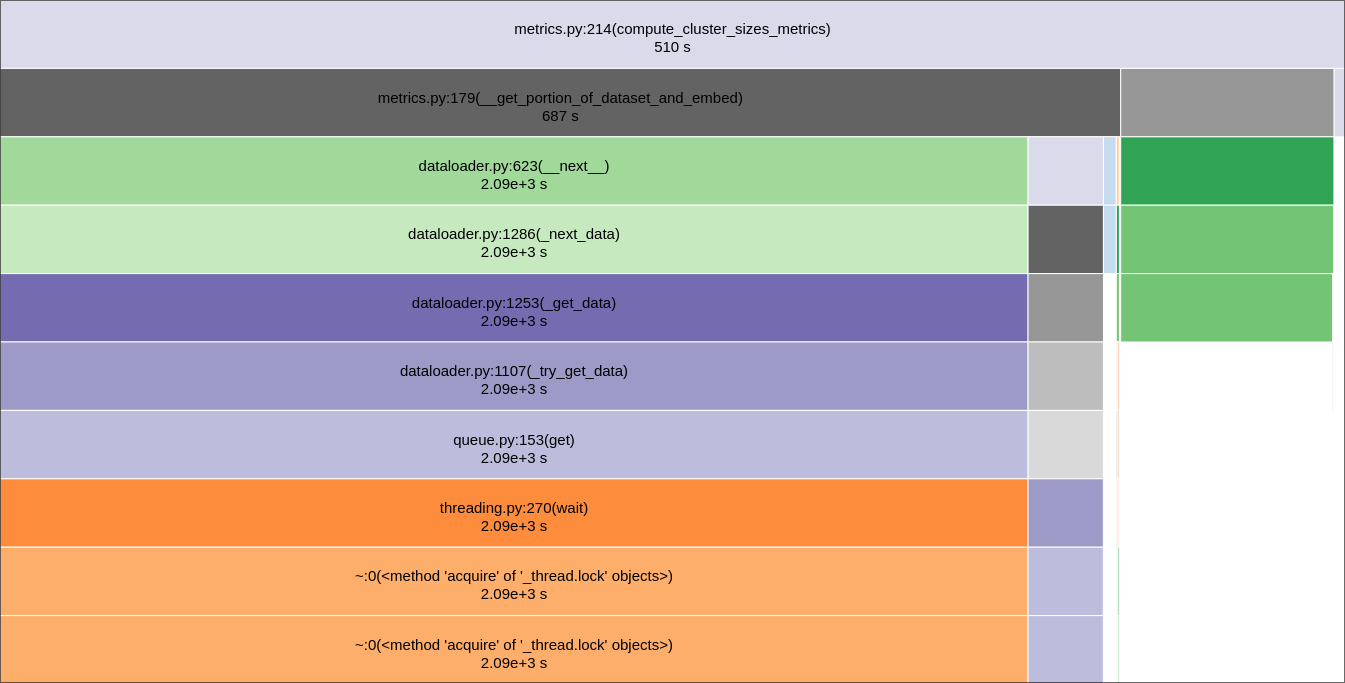
\includegraphics[width=0.98\linewidth]{informatica/profiles/third_profile/logging_segundo}
		\caption{\lstinline{compute_cluster_sizes_metrics}}
	\end{subfigure}

	\begin{subfigure}{.7\textwidth}
		\centering
		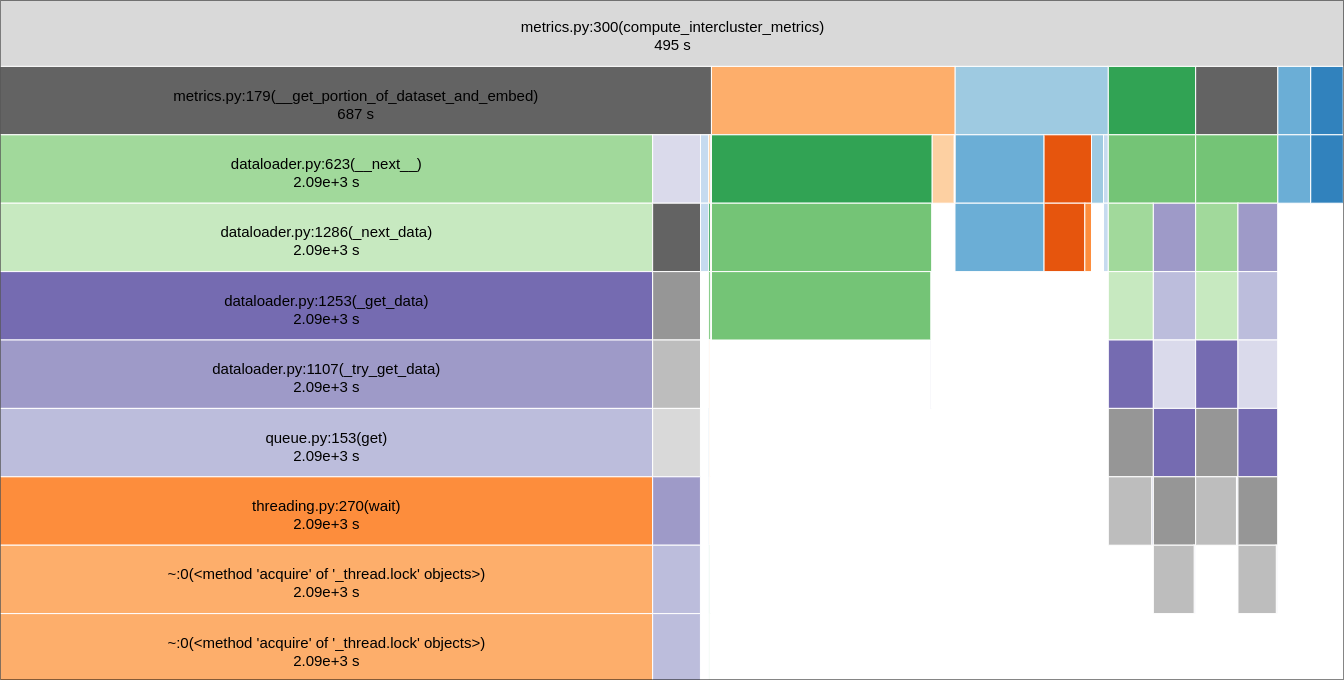
\includegraphics[width=0.8\linewidth]{informatica/profiles/third_profile/logging_tercero}
		\caption{\lstinline{compute_intercluster_metrics}}
	\end{subfigure}
	\caption{Visualización de los tiempos de cómputo asociados a cada una de las tres métricas que mostramos}
	\label{img:optimizacion_05}
\end{figure}

Además, estudiando el archivo con los tiempos de cómputo filtrados \lstinline{./src/profiling/third_profile_filtered.txt}, podemos ver que:

\begin{itemize}
	\item Como ya hemos visto, la mayor parte del tiempo se pasa en \lstinline{log_process}, seguido de \lstinline{calculate_mean_loss_function_online}, \lstinline{__get_portion_of_dataset_and_embed} y \lstinline{compute_cluster_sizes_metrics}.
	\item Una comprensión de diccionarios en \lstinline{precompute_pairwise_distances} supone 1.524 segundos de 1.526 segundos que tarda la función en total.
\end{itemize}

Todo esto justifica que identifiquemos las siguientes partes críticas del código, a tratar en una segunda ronda de optimizaciones:

\begin{itemize}
	\item \lstinline{calculate_mean_loss_function_online}.
	\item \lstinline{__get_portion_of_dataset_and_embed}.
	      \begin{itemize}
		      \item De esta forma, como ya hemos visto previamente, estaríamos optimizando tanto \lstinline{compute_cluster_sizes_metrics} y \lstinline{compute_intercluster_metrics}.
	      \end{itemize}
	\item Mejorar la comprensión de diccionarios en \lstinline{__compute_pairwise_distances}.
\end{itemize}

\section{Segunda ronda de optimizaciones} \label{isubs:segunda_ronda_optimizaciones}

Seguimos el mismo enfoque que en la primera ronda de optimizaciones. Ya tenemos un \textit{benchmark} para \lstinline{compute_intercluster_metrics}. Como \lstinline{compute_intercluster_distances} se usa en \lstinline{compute_intercluster_metrics}, no añadimos un nuevo \textit{benchmark}, y veremos el impacto de los cambios a través del primer \textit{benchmark}.

\begin{table}[!hbtp]
	\centering
	\scalebox{0.8}{
		\begin{tabular}{lccccc}
			\toprule
			\textbf{}           & \multicolumn{2}{c}{\textbf{\lstinline|compute_intercluster_metrics|}} & \multicolumn{2}{c}{\textbf{\lstinline|precompute_pairwise_distances|}} & \textbf{Tiempo entrenamiento}                         \\
			\cmidrule(lr){2-3} \cmidrule(lr){4-5}
			\textbf{Id. Cambio} & Media                                                                 & Desv. Típica                                                           & Media                         & Desv. Típica &        \\
			\midrule
			1                   & 2.55                                                                  & 1.61                                                                   & 12.75                         & 1.48         & 625.89 \\
			2                   & 3.03                                                                  & 1.90                                                                   & 13.62                         & 0.50         & -      \\
			3                   & 3.45                                                                  & 2.68                                                                   & 13.28                         & 0.37         & -      \\
			\bottomrule
		\end{tabular}
	}
	\caption{Tabla que recoge el segundo proceso de optimización del código. Identificamos numéricamente los cambios realizados, que a continuación describiremos. Por cada cambio, vemos los nuevos resultados en los \textit{benchmarks}. También vemos el tiempo que tarda en completarse el ciclo de entrenamiento. Los tiempos de los \textit{benchmarks} se dan como un par (media, desviación típica). Damos los tiempos en segundos}
	\label{table:optimization_process_second}
\end{table}

Describimos los cambios realizados:

\begin{enumerate}
	\item Estado inicial de la base de datos. No se han realizado cambios todavía. Los tiempos en este estado se toman como base a mejorar.
	\item Refactorizamos \lstinline{__get_portion_of_dataset_and_embed} para usar una única llamada de \lstinline{pytorch} para computar todos los \textit{embeddings}, en vez de usar un bucle \lstinline{for}..
	\item Mejoramos el diseño de la anterior función. No deberían producirse cambios en el rendimiento.
\end{enumerate}

En la \tableref{table:optimization_process_second} podemos ver que no estamos mostrando tiempos de cómputo de entrenamiento en las dos últimas entradas. Esto es porque el uso de la función de \lstinline{pytorch} para computar todos los \textit{embeddings} de golpe provoca que el consumo de memoria se eleve hasta abortar el proceso. Además, los \textit{benchmarks} han empeorado algo.

Sin embargo, mantenemos las dos implementaciones, permitiendo elegir cuál usar en cada momento. Puede ser que al acceder a los servidores \textit{nGPU} (véase la \sectionref{isec:entorno_ejecucion}), mucho más potentes, la nueva implementación no provoque consumos elevados de memoria y acelere el proceso.

\section{Comentarios y mejoras a tener en cuenta}

En el momento de realizar este proceso de optimización, no teníamos acceso a los servidores \textit{nGPU}. Sin embargo, era necesario optimizar el código para seguir avanzando el proyecto sin detenernos.

El haber realizado la optimización sobre \textit{Google Colab} y no sobre los servidores \textit{nGPU} sobre los que finalmente correremos el aprendizaje y validación de modelos es un \textbf{error a tener en cuenta}. Por ejemplo, en el \sectionref{isubs:segunda_ronda_optimizaciones} podemos ver que las conclusiones no son del todo robustas al trabajar en un entorno inferior y ser conocedores de que en futuro usaríamos un entorno mucho más potente. Por tanto, \textbf{una posible mejora} es repetir el proceso de optimización sobre los servidores \textit{nGPU}.

Sin embargo, al acceder a los servidores \textit{nGPU} y \textit{datasets} más grandes, no hemos tenido problemas de rendimiento. Con ello, un esfuerzo en optimizar el código no estaría del todo justificado. Por tanto, aún con los fallos que hemos comentado, \textbf{el proceso de optimización cumplió con su cometido} en el momento en el que era necesario.

